\chapter{Experimental Work}
\section{Introduction}
During the research of the related work, many questions arise. The papers are usually very brief and they miss a lot of implementation details. Sadly, even if we tried to contact the authors, we did not get the original source code for the described methods nor for the described benchmarks. The only exception is the \textit{GIRAS} method where we were successful in contacting its author and we do have the complete implementation.\\

All the benchmarks we mentioned in the previous chapter were a part of the papers which describe each particular method. Knowing that we cannot be much surprised that the each presented method outperformed the others. The question is whether we do get the same results on different data sets.\\

The other interesting question is how the winners of the various benchmarks would perform on the same data set. For example, when \textit{GString} outperforms the \textit{C-tree} just by few percents in \cite{GString} and \textit{GraphGrepSX} outperforms \textit{C-tree} by two levels of magnitude, we cannot implicitly say that \textit{GraphGrepSX} would outperform \textit{GString}. There might be three reasons why this presumption might be wrong:

\begin{itemize}
	\item The lack of knowledge of the tested data set. In most the papers there is an information which dataset has been used. On the other hand, there is usually no information about which part of the dataset has been used since the dataset is usually cut down to only a small part of the original size. Moreover, not all the benchmarks are using the same datasets at all.
	
	\item The lack of knowledge about the implementation of the verification step. In non of the mentioned papers is an information about which algorithm has been used for the final subgraph isomorphism testing. This can cause quite a significant difference in the final query measurements (although it cannot influence in the candidate set time computing).
	
	\item We do not even know how much time the authors spent on the optimization of the code itself. Whether they cared more about the code readability and maintainability of the code or whether they did try to optimize the code as much as possible. Moreover, we do not know anything about which languages and compilers have been used.
\end{itemize}

What we did not find at all is some comparison of the performance of the described indexing techniques and utilization of SQL or NOSQL databases. It might be interesting see how significant difference in performance we get when we use very graph specific technique comparing to the very generic ones which the databases offers.\\

In the following sections we will describe what hypotheses do we found interesting to prove or disprove and we describe the process and the implementation of those proves.\\

What is probably fair to mention is that due to the brevity of the related work we cannot be sure whether we did not omit some important part of the algorithms. There has been a lot a situations where we had to improvise since we found out that some very important implementation detail has been omitted in the method descriptions. These cases will be described in following sections as well. Although, we did implement all the methods with opened mind without any endeavor to make some method better or worse, we cannot guarantee that we did not do any mistake or bad implementation decision which can influence the final benchmark results.

\section{Hypotheses to be verified by the experimental work}

In this section we will list several hypotheses which came to our mind during the related work research.

\subsection{Hypothesis 1: GString vs GraphGrepSX}

\textit{GString} and \textit{GraphGrepSX} are using very similar data structures for indexing the database. The main difference is that \textit{GraphGrepSX} is using all graph paths, \textit{GString} is using all paths in the condensed graph. Also \textit{GString} is using heuristics which are very specific for the our field of research, i.e. the organic chemical databases.\\

That being said, we would expect that the index size of \textit{GString} will be significantly smaller due to the condensed graph usage. Also we would expect that due to the specificity of \textit{GString}, it should outperform \textit{GraphGrepSX} which can be used for any graph dataset.

\subsection{Hypothesis 2: GIRAS performance for large queries}

For small queries (of size 4 and 8) the performance of \textit{GIRAS} is about the same as \textit{C-tree}. On the other hand, for larger queries, the performance is ten times better comparing to \textit{C-tree} and even better results are there for the candidate set sizes. What we may question is how it will perform comparing to \textit{GString} and \textit{GraphGrepSX}. From the benchmarks comparisons we may say that \textit{GraphGrepSX} would be the winner. On the other hand the candidate set size should be much better for \textit{GIRAS}. Our guess is that despite the better candidate set size \textit{GIRAS} will not perform better than \textit{GraphGrepSX}.\\

Also, what might be interesting to measure is the index building time for \textit{GIRAS} since it is not mentioned in the paper and the algorithm seems quite computationally complicated.

\subsection{Hypothesis 3: How the SQL and NoSQL databases perform in comparison with the domain specific solutions}

We may question what performance we may get when we use some SQL or NoSQL database. In this case we do not need to implement any special algorithms for index building, we just use the possibilities of the databases, i.e. create a query which describes the subgraph and in case of SQL databases to build the indices to help the query process.\\

We expect that the domain specific indexes will perform much better. But it might be very interesting to see how significant is the performance gap. Also, we may expect that NoSQL databases will perform better compared to the SQL databases since they are usually optimized for storing and querying graphs.

\section{Description of the Experimental Work}

In this section we will describe the implementation details of the experimental work. Based on the uttered hypotheses we have implemented:

\begin{itemize}
	\item \textit{GraphGrepSX} and \textit{GString} algorithms
	
	\item Adapter for the \textit{GIRAS} implementation obtained from Dr. Azaouzi to be working on the same dataset
	
	\item Tools for inserting and querying the SQL and NoSQL database
\end{itemize}

All the implementation has been written in Java language\cite{java}. Most of the work is using Java version 10, NoSQL database adapter is using Java version 8 due to the technology dependencies.\\

For the chemical database parsing we are using Chemistry Development \break Kit\cite{CDK} version 2.1.1, a Java library for working with chemical formats and data structures.\\

In case of verification step for the \textit{GraphGrepSX} and \textit{GString} algorithms, we are using the \textit{SMARTSQueryTool} from Chemistry Development Kit. It uses the \textit{Ullmann}\cite{Ullmann} algorithm inside.

\subsection{GraphGrepSX} \label{graphgrep-implementation}

Since the \textit{GraphGrepSX} algorithm is very simple, the implementation was quite straight-forward.\\

We had to do only one change in the algorithm to make it applicable to our use-case. The original description of the algorithm expects that the suffix tree represents the vertex label paths. Since we need to represent even the edge labels we have changed the original suffix tree presumption so that the odd levels of the suffix tree represent the vertices and the even levels of the suffix tree represent the edges.\\

The previous statement does not affect the {maximum path length parameter $l$ of \textit{GraphGrepSX} algorithm. It is still valid that this parameter sets the maximum length of the index path with regards to the number of vertices, therefore the index tree will have depth up to $2l - 1$.

\subsection{GString}

In contrary to the previous paragraphs, the \textit{GString} algorithm description offers a wide range of pieces which were not described at all. The most of the unknown parts are related to the original graph reduction process where the graph representing the atoms and bonds is transformed into a graph consists only from nodes representing cycles, stars and paths and edges represent just the connection between these structures.\\

The first issue which we faced was the process of extracting the cycles from the original graph. In the algorithm description there are no references on how to extract the cycles nor which method should be used. The obvious issue is that the cycles are not necessarily independent. They can share both vertices and edges and in some cases the vertices and edges can be shared even by several cycles.\\

After some research we have found out that the Chemistry Development Kit has an utility for retrieving \textit{MCB - Minimum Cycle Basis} (also known as \textit{SSSR - Smallest Set of Smallest Rings}) described in \cite{Bauer}. \textit{Cycle Basis} is defined as a set of cycles by which you can express any other cycle present in particular graph as an result a symmetric difference operation on the basis.\\

The \textit{MCB} is defined as a cycle basis which consists of the shortest possible cycles. A good example might be naphthalene which you can see on Figure~\ref{fig:naphthalene}. It contains three cycles, two of size 6 and one of size 10, and any couple of these can serve as a cycle basis. On the other hand, there is only one \textit{MCB} which consist of two cycles of the size 6.\\

On this picture it is also clearly visible why we cannot use all the cycles. If all three cycles would be represented in \textit{GString} graph, it would be very unclear what is the the relationship between these cycles and how they should be connected in \textit{GString} graph. Also, it may lead to false positives from chemistry point of view because naphthalene consist of two aromatic cycles and it does not make sense to include an information about the cycle of the size 10.

\begin{figure}[h]
	\centering
	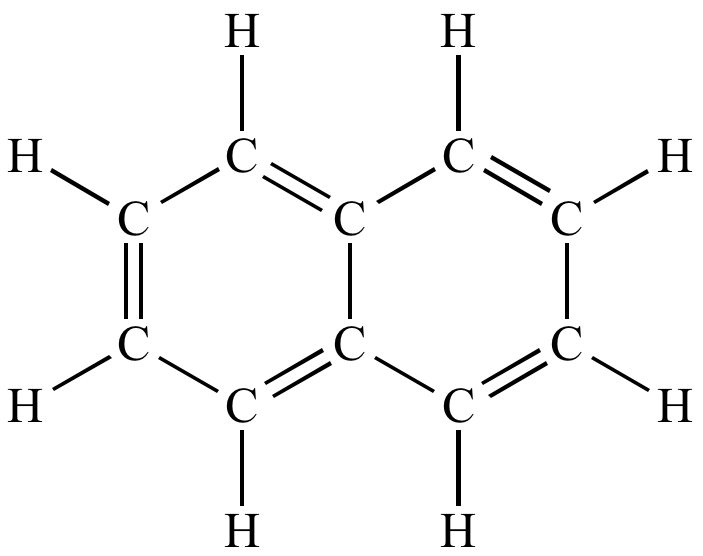
\includegraphics[width=0.25\textwidth]{../img/naphthalene01.png}
	\caption{Molecule of Naphthalene}
	\label{fig:naphthalene}
\end{figure}

The \textit{MCB} finder utility requires specification of the maximum cycle size parameter. This parameter defines a threshold above which the cycles are not considered as cycles. When we tried to set this threshold high enough to not omit any cycle in the testing database, we had big issues with performance and in some cases the process dies on the lack of memory. Since the target of this thesis is to measure the performance in usual use-cases, we have decided to set the threshold to 10 which should cover the vast majority of real cases.\\

Bigger cycles are described as paths of the length equal to the cycle size. These paths begin at each point in which the cycle interfere with another \textit{GString} structure. For each such interference there is are two paths, one in each direction\\

Another question which arose is how to set the threshold which defines the minimum degree of an atom to be considered as star. The original thought was to set the threshold to 3. The reason was that if we set this threshold to higher number we get another problem to solve - how to handle path joints. We can demonstrate this problem on methyl propionate on Figure~\ref{fig:methyl-propionate}\\

\begin{figure}[h]
	\centering
	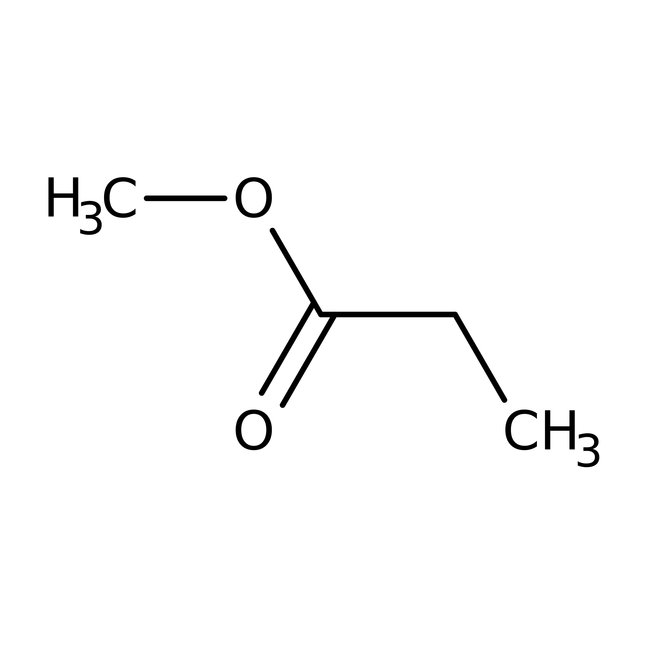
\includegraphics[width=0.25\textwidth]{../img/methyl-propionate.jpg}
	\caption{Molecule of Methyl Propionate}
	\label{fig:methyl-propionate}
\end{figure}

We can see that there are six possible paths, two are between the carbons (one from each side), and four between each carbon and oxygen (again, one from each side). If we define the threshold of stars to three, we do not have to handle such situations because in our algorithm, we extract the stars first and then we are finding paths connected to already found stars and cycles. In this case we would have 1 star (the atom in the middle) and two paths connected to it (the oxygen connected by double bond would be considered as a branch which is by definition a path of length 1). This would simplify the algorithm quite a lot because we would not need to handle paths which are connected to another paths.\\

During the testing we found out that it is possible to use this threshold but in practice, we would lost majority of results. The reason is the same as we described in the first chapter. If we try to query a path which may be described as $C-O-C-C-C$ there is obviously such path in methyl propionate but our algorithm would filter this candidate out because it does not contain a path of size 5 but a star and two paths of length 2. Since this is a very common use-case we had to use higher threshold and develop some logic for handling the connected paths.\\

What we did was to implement DFS which finds all the paths and all of these paths are included into the \textit{GString} graph. In case of methyl propionate there would be 2 independent paths, since we do not have a connection to any other structure, we start DFS in random atom with degree 1. This is quite a special case because the molecule consist only of paths. If the methyl propionate would be connected on one end to star or cycle, there would be 2 nodes in the \textit{GString} graph - one cycle/star and two paths connected to this structure.\\

The rest of the algorithm mimics the \textit{GraphGrepSX} implementation including the notes described in \ref{graphgrep-implementation}.

\subsection{SQL Database}

We have based our implementation on the proposal in \cite{SQL}. We have chosen the Oracle Database 12c. For the Java API we have used Oracle Database JDBC driver 12.2.0.1.\\

Based on the mentioned paper we have designed our table with 5 columns - \textbf{ATOM1\_ID}, \textbf{ATOM2\_ID}, \textbf{BOND\_ID}, \textbf{BOND\_TYPE} and \break \textbf{COMPOUND\_ID}.\\


The implementation itself is quite straightforward and it consist of two parts. The first part is a routine for the database creation. In this routine we just iterate through the whole database and for each molecule, at first, we iterate through all its atoms and assign an unique ID to each of them, later, we iterate through all the bonds and for each we create one \textbf{INSERT} statement.\\

We already have the IDs of atoms and compound ID (this comes from the original chemical DB on the input), we generate an unique ID for bond itself. Type of bond consists of the type of each atom at the bond's end and the type of the bond itself. Each bond, if it is not symmetrical, is represented by two rows in the database because we need to make the graph representation undirected. During the process of inserting the bonds we are updating the in-memory statistics - we are maintaining the count of rows for each bond type.\\

The inserts are happening in batches. We did test the performance and found out that batch size of 50 rows for one \textbf{INSERT} statement is quite optimal.\\

The second part of the implementation is the query building. As proposed in \cite{SQL}, at first we build the minimal spanning tree of the query graph. The edge value is based on the database statistics which we gather during the insert phase. For spanning tree construction we have implemented Kruskal algorithm.\\

Then, in the spanning tree we find the edge with lowest value and from this edge we start a BFS algorithm and for each edge we add the rule into the \textbf{SELECT} statement. We also need to mark all the neighbours by stating that atom ID of one edge is equal to the atom ID of the neighbour edge. The same we have to do for non-neighbours. For each such pair we have to explicitly state that their atom IDs are not equal. The same we have to do for the bonds, we need all the bonds unique so we have to state for each pair of bonds that their IDs are not equal.\\

Since we are interested only in the information whether the subgraph is present in particular compound, we start our \textbf{SELECT} statement with \textbf{SELECT DISTINCT b0.COMPOUND\_ID FROM ...} which returns the set of compounds matching the subgraph query which is exactly the result we need.

\subsection{NoSQL Database}

\subsection{GIRAS}

As we were successful with the request of the original implementation of \textit{GIRAS} algorithm, there was not much implementation needed on the side of this thesis. For the measurement we are using the original solution. We had to implement only an adapter which translates the chemical database which we are using for other methods to the format - vertex and edge lists - accepted by the \textit{GIRAS} code.\\

However, during the testing we have found out that the results are not matching the results of other methods. After some investigation, we have realized that the problem is not in the implementation but in the algorithm itself. The core of the problem is in the way how the structures which are being indexed are chosen.\\

As we mentioned in the analysis chapter, \textit{GIRAS} method is trying to find the rare substructures with the condition that every graph in the database has to be represented by at least one rare subgraph. We have found out that when we create a query which should have only several results, everything works fine. On the other hand when we build a query which should match nearly whole database, we do not get any results at all.\\

We did an explicit test which proves that the algorithm cannot work properly in all cases. We have created a database with 4 molecules where each of them contain a path of four aromatic carbons but in each of them there is a unique substructure which do not contain this particular path.\\

When we have executed a query of the mentioned path we did not get any results. When we have added new molecule into the database which represents the query itself, i.e. path of four aromatic carbons, and we ran the query again, the result was that the query matches all the graphs in the database.\\

This observation invalidates the statement in \cite{GIRAS} that the indexing is complete. We may then question how the results of the performance measurements are valid. If we know that the indexing is incomplete, it should be also faster since the index is smaller and therefore it should take less time to use it. So even for the queries which results are valid, we may question how seriously we can take the performance numbers.